\documentclass{beamer}
\usepackage[utf8]{inputenc}
\usepackage{graphicx, fancyhdr, amsmath, amssymb, hyperref, esint, listings, color, caption, afterpage, float, nicematrix, soul, physics, simpler-wick, nccmath, framed, tcolorbox, pifont}
\usepackage[dvipsnames]{xcolor}

\usetheme{Berlin}
\usecolortheme{wolverine}
\usepackage{ragged2e}
\usepackage{enumitem}
\setlist[itemize]{left=0em, label={\color{blue}\ding{49}}, font=\color{red}}
\newcommand{\red}[1]{{\color{red} #1}}
\newcommand{\green}[1]{{\color{ForestGreen} #1}}
\newcommand{\blue}[1]{{\color{blue} #1}}

\setbeamertemplate{navigation symbols}{} %hide the navigation button
%\setbeamercovered{transparent}

\title{Channels, Gaussian Channels and Network Information Theory}
\subtitle{Presentation for (CS1.407) Entropy and Information Course}
\author[Soumit, Damini, Meet] % (optional, for multiple authors)
{Soumit Roy\inst{1} \and Damini Chandi Priya Adusumilli\inst{2} \and Meet Gera\inst{3}}

\institute[IIITH] % (optional)
{
  \inst{1}%
  Ph.D. Student (Roll No: 2023811002), CQST, IIITH
  \and
  \inst{2}%
  DD Student (Roll No: 2023122005), CVEST, IIITH
  \and
  \inst{3}%
  SD Student (Roll No: 2022102039), RRC ,IIITH
}
\logo{
\includegraphics[scale=0.25]{iiit.jpeg}}

\date{\red{\today}}



%%%%%%%%%%%%%%%%%%%%%%%%%%%%%%%%%%%%%%%%%%%%%%%%%%%%%%%%%%%%%%%%%%
\begin{document}


%The next statement creates the title page.
\frame{\titlepage}
%%%%%%%%%%%%%%%%%%%%%%%%%%%%%%%%%%%%%%%%%%%%%%%%%%%%%%%%%%%%%%%%%%
\logo{}
%%%%%%%%%%%%%%%%%%%%%%%%%%%%%%%%%%%%%%%%%%%%%%%%%%%%%%%%%%%%%%%%%%%
%Frame-2 
\begin{frame}
\subsection{Part-I}

\textbf{Plan for Part-I}
\begin{itemize}
    \item Recap of Channels and Channel Capacity
    \item Gaussian Channels
    \item Coding Theorem for Gaussian Channels
\end{itemize}
%
\end{frame}
%%%%%%%%%%%%%%%%%%%%%%%%%%%%%%%%%%%%%%%%%%%%%%%%%%%%%%%%%%%%%%%%%%%

%Frame-3
\section{GC}

\begin{frame}{Gaussian Channels}
 \begin{itemize}
	\justifying

\item<1->  

	\end{itemize}
\end{frame}
%%%%%%%%%%%%%%%%%%%%%%%%%%%%%%%%%%%%%%%%%%%%%%%%%%%%%%%%%%%%%%%%%%%
%Frame-part-ii 
\begin{frame}
\subsection{Part-II}

\textbf{Plan for Part-II}
\begin{itemize}
    \item Parallel Gaussian Channels
    \item Channels with Colored Gaussian Noise
    \item  Gaussian Channels with Feedback
    \item Gaussian Multiple-User Channels
\end{itemize}
%
\end{frame}
%Frame-3
\section{TGC}

\begin{frame}{Parallel Gaussian Channels}
 \begin{itemize}
	\justifying
\item If there are  $k$ common power constaint, guassian channels (NWAGN : non-white additive Guassian Noise channel) which are considered to be independent and in parallel where different frequency is represented by each parallel channel.
\begin{center}
	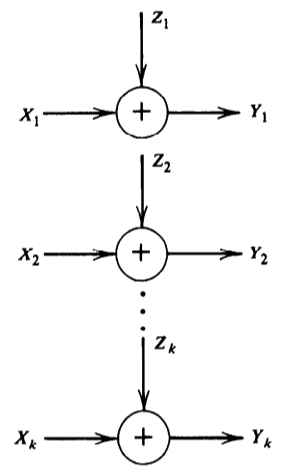
\includegraphics[scale=0.15]{Diagrams/parallel_guassian_channels.png}
\end{center} 
\item Output for channel $j$ , it would be: \begin{eqnarray}
    Y_j = X_j + Z_j, \quad j = 1, 2, \dots, k,
\end{eqnarray}
%

\item The constaint on power can be described as:
%
\begin{eqnarray}
    \mathbb{E} \sum_{j=1}^{k} X_j^2 \leq P
\end{eqnarray}
%


	\end{itemize}
\end{frame}
%%%%%%%%%%%%%%%%%%%%%
\begin{frame}{Parallel Gaussian Channels}
 \begin{itemize}
	\justifying
\item Information capacity of Channel C is given by:
%
\begin{eqnarray}
    C = \max_{f(x_1, x_2, \dots, x_k) : \sum \mathbb{E} X_j^2 \leq P} I(X_1, X_2, \dots, X_k ; Y_1, Y_2, \dots, Y_k)
\end{eqnarray}
\item In order to maximise Capacity , power allotment in the constaint \( \sum P_j = P \) needs to be found, where \( P_j = \mathbb{E} X_j^2 \) 
\item Due to the fact that \( P_j \)'s must be positive,Kuhn-Tucker Conditions can be used to find $v$ such that capacity is maximum.
%
\begin{eqnarray}
    P_j = (\nu - N_j)^+
\end{eqnarray}
%
above $(x)^+$ shows non-negative of $x$ 


	\end{itemize}
\end{frame}
%%%%%%%%%%%%%%%%%%%%%
%%%%%%%%%%%%%%%%%%%%%
\begin{frame}{Water Filling Process}
 \begin{itemize}
	\justifying
\item The picture below gives an graphical representation of a solution , power is alloted to channels as signal power increases from 0 , power is put into channels which are noiser . Like this Power is distributed into various bins and is referred to as $"Water-Filling"$ process.
\begin{center}
	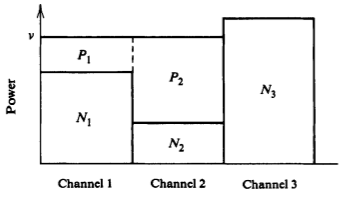
\includegraphics[scale=0.5]{Diagrams/parallel_guassian_channels_solution.png}
\end{center} 


	\end{itemize}
\end{frame}
%%%%%%%%%%%%%%%%%%%%%
%%%%%%%%%%%%%

\begin{frame}{Channels with Colored Gaussian Noise}
 \begin{itemize}
	\justifying
\item Considering $n$ parallel gaussian channels whose noise is dependent , considering the input covariance matrix of input and noise to be $K_x$ and $K_z$ respectively. 
\item The power constaint of input now depends on $n$ and can be seen as,
\begin{equation}
\frac{1}{n} \sum_i \mathbb{E}X_i^2 \leq P,
\end{equation}
\item The Covariance of the output \( Y \) since the input and the noise are independent can be given by \( K_Y = K_X + K_Z \) .
\item we need to maximise \( |\mathbf{A} + \mathbf{\Lambda}| \) , to maximise C , where \( A = Q^T K_X Q \).


	\end{itemize}
\end{frame}
%%%%%%%%%%%%%%%%%%%%%%%%%%%%%%%%%%
%%%%%%%%%%%%%%%%%%%%%%%%%%%%%%%%%%

\begin{frame}{Gaussian Channels with Feedback}
 \begin{itemize}
	\justifying
\item Capacity doesnot change with adding Feedback to DMC but having a Feedback can surely reduce the encoding and decoding complexity.When it comes to Channels with Memory, from time to time the noise gets correlated.
\item The Gaussian channel with feedback can be seen as below ,
\begin{center}
	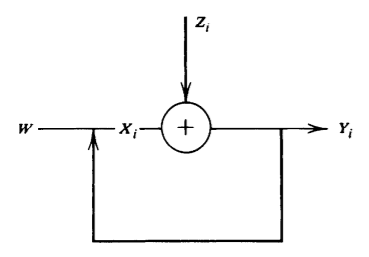
\includegraphics[scale=0.2]{Diagrams/Gaussian_Channel_with_FeedBack.png}
\end{center} 
\item  $Y_i$ which is the output of the channel is given by,
\begin{equation}
Y_i = X_i + Z_i, \quad Z_i \sim \mathcal{N}(0, K_Z^{(i)})
\end{equation}
\item It can be finally concluded that 
\begin{equation}
C_{n,FB} \leq C_n + \frac{1}{2} \text{ bits per transmission} 
\end{equation}


	\end{itemize}
\end{frame}
%%%%%%%%%%%%%%%%%%%%%%%%%%%%%%%%%%
\section{MUC}
\begin{frame}{Multiple User Channels}
 \begin{itemize}
	\justifying
\item The capacity of Gaussian Channel is given by:
\begin{equation}
C = \frac{1}{2} \log \left( 1 + \frac{P}{N} \right) \text{ bits per transmission.}
\end{equation}

Below , are different types of discrete-time memoryless Gaussian channels.
\item Single User Gaussian Channel
Choosing an index \( i \) in the set \( 2^{nR} \) in a codebook \( (2^{nR}, n) \) with rate \( R < \frac{1}{2} \log(1 + \frac{P}{N}) \). \( Y = X(i) + Z \) is observed by the receiver, and from \( Y \), receiver tries to find the index \( i \).
Probability of error \( P_e\) will be arbitrarily small when \( n \) is sufficiently large.



	\end{itemize}
\end{frame}
%%%%%%%%%%%%%%%%%%%%%
\begin{frame}{Multiple User Channels}
 \begin{itemize}
	\justifying
\item  Multiple Access Channel with m Users 
\item The observed output with \( m \) transmitters is:
\begin{equation}
Y = \sum_{i=1}^m X_i + Z.
\end{equation}
\item Extending the single user case above to $m$ users,
\begin{equation}
\sum_{i=1}^m R_i < C \left( \frac{mP}{N} \right).
\end{equation}
Gaussian Channel with \( m \) users can be understood in lines of a single user with a slight difference that there are \( 2^{n R_i} \) codewords within an \( i \)th codebook and there are  \( m \) codebooks .




	\end{itemize}
\end{frame}
%%%%%%%%%%%%%%%%%%%%%
%%%%%%%
\begin{frame}{Multiple User Channels}
 \begin{itemize}
	\justifying
\item    Broadcast Channel 
\item In this type of channel, there are $2$ receivers that are distinct in terms of noise power $ie$ having \( N_1 \) and \( N_2 \) with the same signal power  \( P \). Assuming \( N_1 < N_2 \), then it implies that there is less noise in the receiver $Y1$ when compared to $Y2$, the output of each Gaussian Channel is given by the same formula,
\begin{equation}
Y_1 = X + Z_1  
\end{equation}
\begin{equation}
Y_2 = X + Z_2  
\end{equation}
in the above, it is to note that sender wants to send messages to receivers \( Y_1 \) and \( Y_2 \) at rates \( R_1 \) and \( R_2 \) and that  \( Z_1 \) is a correlated Gaussian RVs with $\mathrm{Var}$ \( N_1 \) and similarly  \( Z_2 \) with $\mathrm{Var}$ \( N_2 \).




	\end{itemize}
\end{frame}
%%%%%%%%%%%%%%%%%%%%%
%%%%%%%
\begin{frame}{Multiple User Channels}
 \begin{itemize}
	\justifying
\item    Relay Channel 
\item In this type of Gaussian Channel, there is a sender $X$ and receiver \( Y \) along with a Relay Channel to help the receiver, the output of the channel is described as :
\begin{equation}
Y_1 = X + Z_1,
\end{equation}
\begin{equation}
Y = X + Z_1 + X_1 + Z_2,
\end{equation}

Encoding by the relay, which is allowed, is 
\begin{equation}
X_1 = f(Y_1, Y_{12}, \ldots, Y_{1, t-1}).
\end{equation} 
and \( Z_1 \) is a independent Gaussian RVs with $\mathrm{Var}$ \( N_1 \) and
$\mu$ as $0$ similarly  \( Z_1 \) with $\mathrm{Var}$ \( N_2 \)  and $\mu$ as $0$.
If the power is $P1$ of sender $X1$ and $P$ of $X$.




	\end{itemize}
\end{frame}
%%%%%%%%%%%%%%%%%%%%%
%%%%%%%
\begin{frame}{Multiple User Channels}
 \begin{itemize}
	\justifying
\item Interference Channel:
\begin{center}
	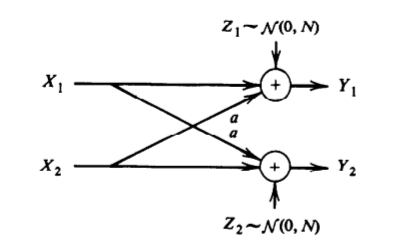
\includegraphics[scale=0.2]{Diagrams/Gaussian_Interference_Channel.png}
\end{center} 
\item This type of channel is quite different from the ones discussed above as it is has $2$ senders and receivers and also sender $1$ sends information only to receiver $1$ and doesnot care about the other receiver understanding, similarly with sender $2$ and receiver $2$.




	\end{itemize}
\end{frame}
%%%%%%%%%%%%%%%%%%%%%
%%%%%%%
\begin{frame}{Multiple User Channels}
 \begin{itemize}
	\justifying
\item    Gaussian Two-Way Channel
\item This Channel is similar to the one discussed above but with a change that Gaussian Two-Way channel has Feedback and here senders of both are attached to the other receiver $ie$ upon understanding the previous received symbols of receiver $2$ , sender $1$ can decide what can be sent next.
\begin{center}
	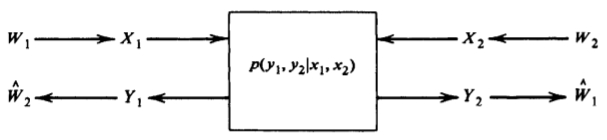
\includegraphics[scale=0.5]{Diagrams/Gaussian_Two-Way_Channel.png}
\end{center} 




	\end{itemize}
\end{frame}
%%%%%%%%%%%%%%%%%%%%%
%%%%%%%%%%%%%%%%%%%%%%%%%%%%%%%%%
{\small
%Frame-part-iii 
\begin{frame}

\subsection{Part-III}

\textbf{Plan for Part-III}
\begin{itemize}
    \item Multiple-Access Channel (MAC)
    \item Achievability of the Capacity Region for the MAC
    \item m-User MACs
    \item Gaussian MAC
    \item Slepian-Wolf Theorem
    \item Broadcast Channel (A Brief Introduction)
\end{itemize}
%
\end{frame}

%%%%%%%%%%%%%%%%%%%%%%%%%%%%%%%%%%%%%%%%%%%%%%%%%%%%%%%%%%%%%%%%%%%
%Frame
\section{MAC}

\begin{frame}{Multiple-Access Channels (MAC)}
 \begin{itemize}
	\justifying

\item<1-> Two or more senders send information to a common receiver. 
\item<2-> \green{Example:} A bunch of cell phones, tabs and laptops communicating with a base station is a prominent example of this channel. \\
\begin{center}
    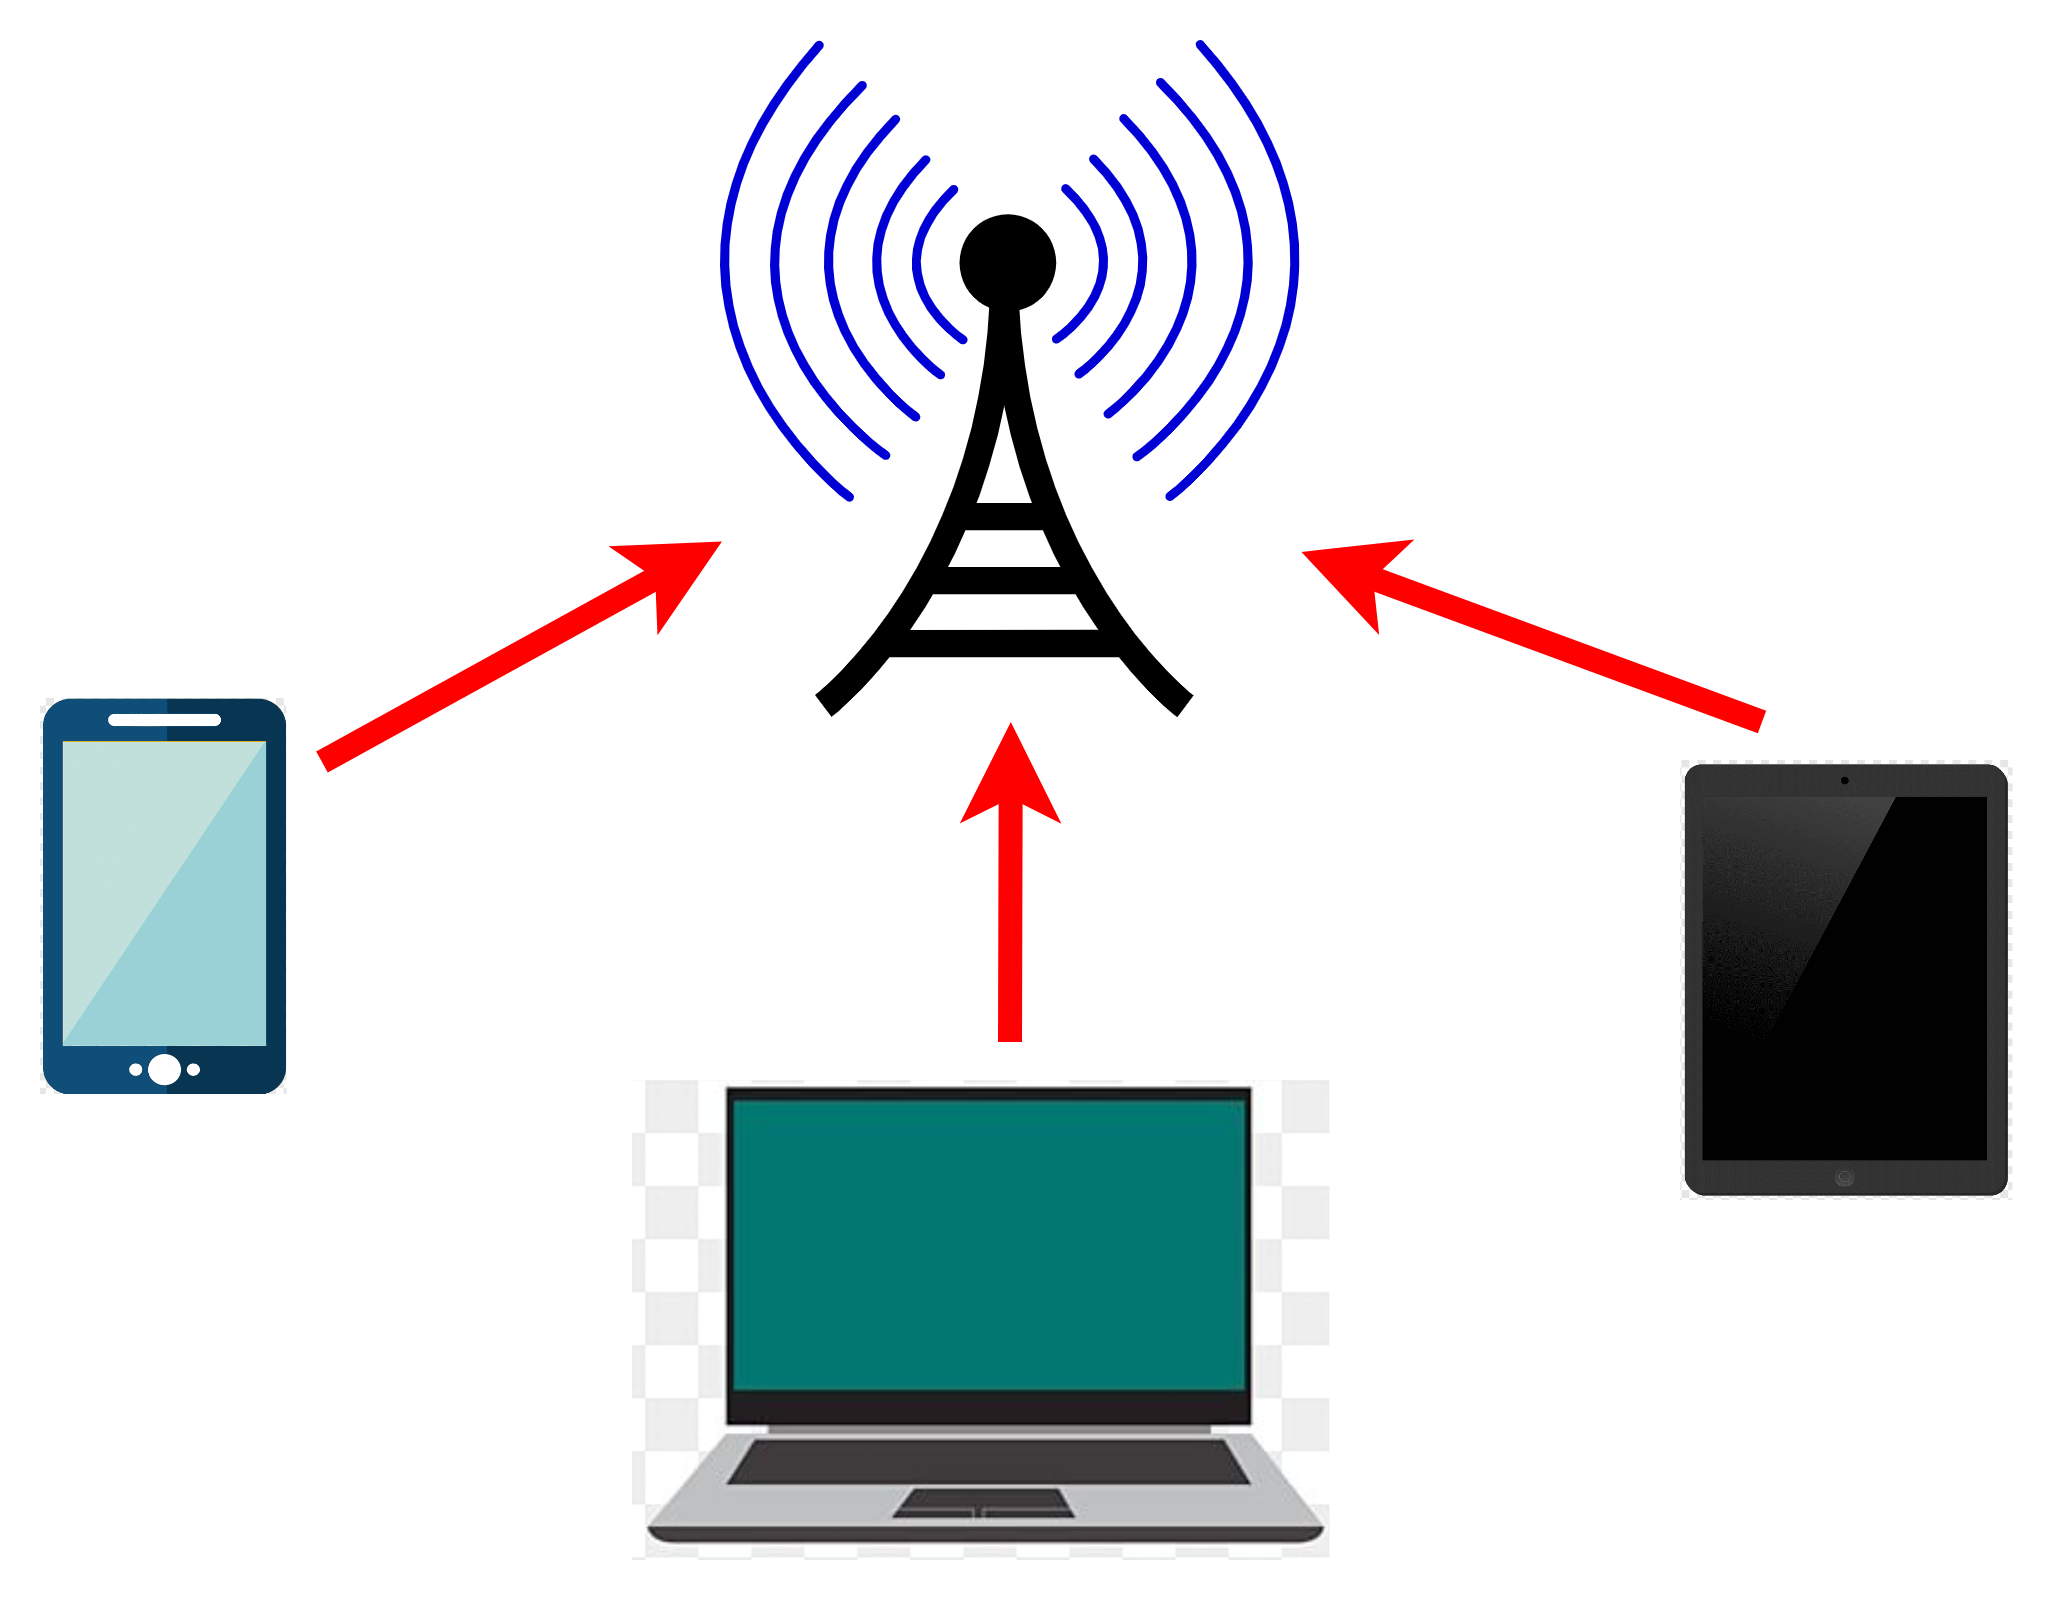
\includegraphics[scale=0.05]{Presentation Diagrams/MAC.png}
\end{center}
%
\item<3-> Senders face the receiver noise \& interference from other senders.  

	\end{itemize}
\end{frame}
%%%%%%%%%%%%%%%%%%%%%%%%%%%%%%%%%%%%%%%%%%%%%%%%%%%%%%%%%%%%%%%%%%%
%Frame
\begin{frame}{Definitions} 

 \begin{itemize}
	\justifying
\item<1-> Let us consider a two-user MAC.
\item<2-> {\color{red}A discrete memoryless multiple-access channel} consists of three alphabets, $\mathcal{X}_1, \mathcal{X}_2,$ and $\mathcal{Y}$, and a probability transition matrix $p(y|x_1,x_2)$.
%
\item<3-> {\color{red} A $((2^{nR_1},2^{nR_2}),n)$ code} for the multiple-access channel consists of two sets of integers $\mathcal{W}_1 = \{1,2,...,2^{nR_1} \}$ and $\mathcal{W}_2 = \{1,2,...,2^{nR_2} \}$, called the message sets, two encoding functions,
%
\begin{eqnarray*}
    X_1: \mathcal{W}_1 \rightarrow \mathcal{X}_1^n, \text{ and } X_2: \mathcal{W}_2 \rightarrow \mathcal{X}_2^n,
\end{eqnarray*}
%
and a decoding function $g: \mathcal{Y}^n \rightarrow \mathcal{W}_1 \times \mathcal{W}_2.$  
	\end{itemize}
\end{frame}
%%%%%%%%%%%%%%%%%%%%%%%%%%%%%%%%%%%%%%%%%%%%%%%%%%%%%%%%%%%%%%%%%%%
%Frame
\begin{frame}%{Definitions (Contd.)} 
\begin{center}
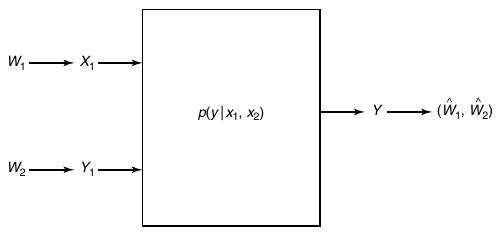
\includegraphics[scale=0.35]{Diagrams/MAC.png}    
\end{center}
%
 \begin{itemize}
	\justifying

\item<1-> Sender 1 (Sender 2) chooses an index $W_1$ uniformly from the set $\{1,2,...,2^{nR_1}\}$ ($\{1,2,...,2^{nR_2}\}$) and sends the codeword over the channel. 

\item<2-> Assume that the messages are independent and equally likely \textit{i.e.} the distribution of messages over the product set $\mathcal{W}_1 \times \mathcal{W}_2$ is uniform.

\item<3-> \red{The average probability of error} for the $((2^{nR_1},2^{nR_2}),n)$ code is given by
%
\begin{eqnarray*}
    P_e^{(n)} = \frac{1}{2^{n(R_1+R_2)}} \sum_{(w_1,w_2)\in \mathcal{W}_1 \times \mathcal{W}_2}\Pr {g(Y^n) \neq (w_1, w_2)|(w_1, w_2) \quad \text{sent}}.
\end{eqnarray*}
% 

 \end{itemize}
\end{frame}
%%%%%%%%%%%%%%%%%%%%%%%%%%%%%%%%%%%%%%%%%%%%%%%%%%%%%%%%%%%%%%%%%%%
%Frame
\begin{frame}{Achievable Rate Pair and The Capacity Region} 
%
 \begin{itemize}
	\justifying

\item<1-> \red{A rate pair $(R_1, R_2)$} is said to be achievable for the multiple-access channel if there exists a sequence of $((2^{nR_1},2^{nR_2}),n)$ codes with $P_e^{(n)}\rightarrow 0$.

\item<2->  \red{The capacity region} of the multiple-access channel is the closure of the set of achievable $(R_1, R_2)$ rate pairs.

\item<3-> \begin{tcolorbox}[colback=blue!10, colframe=blue, title=Theorem for Capacity Region of MAC]
The capacity of a multiple-access channel $(\mathcal{X}_1 \times \mathcal{X}_2, p(y|x_1,x_2), \mathcal{Y})$ is the closure of the convex hull of all $(R_1, R_2)$ satisfying
%
\begin{eqnarray*}
    R_1 < I(X_1; Y|X_2); \text{ }  R_2 < I(X_2; Y|X_1); \text{ } 
    R_1+R_2 < I(X_1, X_2; Y)
\end{eqnarray*}
%
for some product distribution $p(x_1)p(x_2)$ on $\mathcal{X}_1 \times \mathcal{X}_2$.
\end{tcolorbox}
	\end{itemize}
\end{frame}
%%%%%%%%%%%%%%%%%%%%%%%%%%%%%%%%%%%%%%%%%%%%%%%%%%%%%%%%%%%%%%%%%%%
%Frame
\begin{frame}{Different Capacity Region for MAC} 
\begin{center}
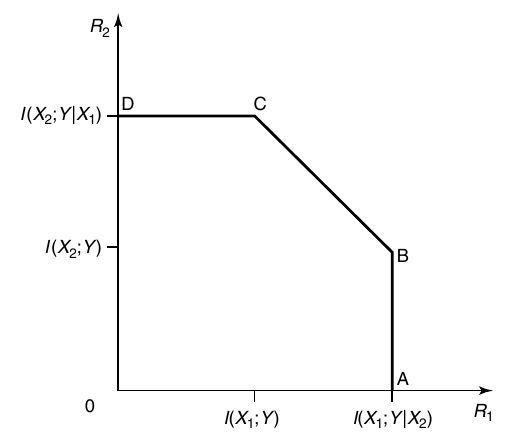
\includegraphics[scale=0.4]{Diagrams/Achievable region of MAC.png}    
\end{center}
%
\end{frame}

%%%%%%%%%%%%%%%%%%%%%%%%%%%%%%%%%%%%%%%%%%%%%%%%%%%%%%%%%%%%%%%%%%%
%Frame
\begin{frame}
%
 \begin{itemize}
	\justifying

\item<1-> \blue{\textbf{Point A:}} Sender 2 is not sending any information. Therefore, the maximum rate is achievable due to sender 1. Therefore for any distribution $p_1(x_1)p_2(x_2)$,
    %
    \begin{eqnarray*}
        \max R_1 = \max_{p_1(x_1)p_2(x_2)}  I(X_1;Y|X_2)= \max_{x_2}  I(X_1;Y|X_2=x_2),
    \end{eqnarray*}
    %
    \textit{i.e.}, maximum is attained when we set $X_2 = x_2$.

\item<2-> \blue{\textbf{Point B:}} If $X_1$ is regarded as noise for the channel from $X_2$ to $Y$, this is the rate that is achieved. The obtained rate is
    %
    \begin{eqnarray*}
        \sum_{x_2} p(x_2)I(X_1;Y|X_2 = x_2) = I(X_1;Y|X_2).
    \end{eqnarray*}

\item<3-> \blue{\textbf{Point C:}} This point corresponds to point B, where the receiver and sender roles are interchanged.

\item<4-> \blue{\textbf{Point D:}} This point corresponds to point A, where the receiver and sender roles are interchanged.
    \end{itemize}
    %

\end{frame}
%%%%%%%%%%%%%%%%%%%%%%%%%%%%%%%%%%%%%%%%%%%%%%%%%%%%%%%%%%%%%%%%%%%
%Frame
\begin{frame}{$m$-user MAC}
%
 \begin{itemize}
	\justifying

\item<1-> Generalized version of the MAC with $m \geq 2$.

\item<2-> The sender $1,2,...,m$ sends the independent indices $w_1,w_2,...,w_m$ over the channel respectively. 

\item<3-> The codes, rates, and achievability are defined in exactly the same way.
\begin{center}
    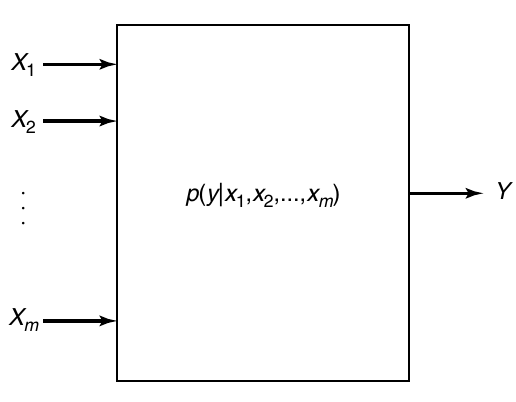
\includegraphics[scale = 0.25]{Diagrams/M-user MAC.png}
\end{center}
    \end{itemize}
   %

\end{frame}
%%%%%%%%%%%%%%%%%%%%%%%%%%%%%%%%%%%%%%%%%%%%%%%%%%%%%%%%%%%%%%%%%%%%
%Frame
\begin{frame}{$m$-user MAC} 

\begin{itemize}
\item<1-> \begin{tcolorbox}[colback=blue!10, colframe=blue, title=Theorem for Capacity Region of $m$-MAC]
Let $S \subseteq \{1,2,...,m\}$ and $S^c$ denote the complement of $S$. Let $R(S)=\sum_{i \in S} R_i$, and let $X(S)=\{X_i: I \in S \}$. Then, the capacity region of the $m$-user multiple-access channel is the closure of the convex hull of the rate vectors satisfying
%
\begin{eqnarray*}
    R(S) \leq I(X(S);Y|X(S^c)) \quad \forall S \subset \{1,2,...,m\}
\end{eqnarray*}
%
for some product distribution $p_1(x_1)p_2(x_2)...p_m(x_m)$.
\end{tcolorbox}
    \end{itemize}

\end{frame}
%%%%%%%%%%%%%%%%%%%%%%%%%%%%%%%%%%%%%%%%%%%%%%%%%%%%%%%%%%%%%%%%%%%
%Frame
\section{GMAC}

\begin{frame}{Gaussian MAC}
 \begin{itemize}
	\justifying

\item<1-> Consider two senders, $X_1$ and $X_2$, who communicate to the single receiver, $Y$. The received signal at time $i$ is
%
\begin{eqnarray*}
    Y_i = X_{1i}+X_{2i}+Z_i,
\end{eqnarray*}
%
where $\{Z_i\}$ is a sequence of i.i.d., zero mean Gaussian random variables with variance $N$.

\begin{center}
    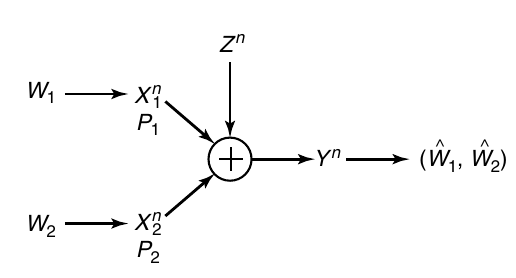
\includegraphics[scale = 0.3]{Diagrams/GMAC.png}
\end{center}

	\end{itemize}
\end{frame}
%%%%%%%%%%%%%%%%%%%%%%%%%%%%%%%%%%%%%%%%%%%%%%%%%%%%%%%%%%%%%%%%%%%
%Frame
\begin{frame}
 \begin{itemize}
	\justifying

\item<1-> Different power constraints for different senders.

\item<2-> $P_j$ be the power constraint associated with the sender $j$, \textit{i.e.} for each sender and all messages we must have,
%
\begin{eqnarray*}
    \frac{1}{n} \sum_{i = 1}^n x^2_{ij} (w_j) \leq P_j, \quad w_j \in \{1,2,...,2^{nR_j}\}, \quad j = 1,2.
\end{eqnarray*} 

\item<3-> Mutual information in terms of relative entropy \textit{i.e.}
%
\begin{eqnarray*}
    I(X_1;Y|X_2) \leq \frac{1}{2}\log(1+\frac{P_1}{N}) &:=& C\left(\frac{P_1}{N} \right) \\
    I(X_1;Y) \leq \frac{1}{2}\log(1+\frac{P_1}{P_2+N}) &:=& C\left(\frac{P_1}{P_2+N}\right)
\end{eqnarray*}
%

	\end{itemize}
\end{frame}
%%%%%%%%%%%%%%%%%%%%%%%%%%%%%%%%%%%%%%%%%%%%%%%%%%%%%%%%%%%%%%%%%%%%
%Frame
\begin{frame}{Capacity Pentagon for Gaussian MAC}
 \begin{itemize}
	\justifying

\item<1-> \begin{tcolorbox}[colback=blue!10, colframe=blue, title=Capacity Region of GMAC]
The bound on $R_1$, $R_2$ and $R_1+R_2$ for a Gaussian MAC is
%
\begin{eqnarray*}
    R_1 \leq C\left(\frac{P_1}{N}\right); \text{ } R_2 &\leq& C\left(\frac{P_2}{N}\right); \text{ }  R_1+R_2 \leq C\left(\frac{P_1+P_2}{N}\right)
\end{eqnarray*}
%
for some product distribution $p(x_1)(x_2)$ on $\mathcal{X}_1 \times \mathcal{X}_2$.
\end{tcolorbox}
%
\item<2-> Equality is achieved when $X_1 \sim \mathcal{N}(0,P_1)$ and $X_2 \sim \mathcal{N}(0,P_2)$.

	\end{itemize}
\end{frame}
%%%%%%%%%%%%%%%%%%%%%%%%%%%%%%%%%%%%%%%%%%%%%%%%%%%%%%%%%%%%%%%%%%%%
%Frame
\begin{frame}
\begin{center}
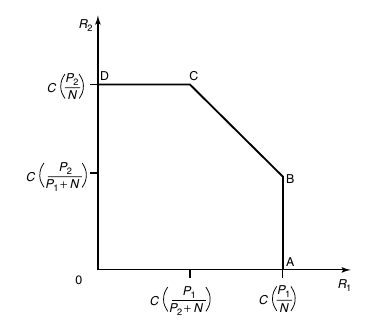
\includegraphics[scale=0.55]{Diagrams/GMACC.png}    
\end{center}
%
\end{frame}
%%%%%%%%%%%%%%%%%%%%%%%%%%%%%%%%%%%%%%%%%%%%%%%%%%%%%%%%%%%%%%%%%%%
%Frame
\begin{frame}{The Interpretation}
 \begin{itemize}
	\justifying

\item<1-> The interpretation is almost equivalent to the case described for a general MAC  for a fixed distribution. 

\item<2-> The decoding process AKA \blue{Onion-Peeling}:
\begin{itemize}
    \item  \textbf{The First Stage:} The receiver decodes the second sender, considering the first sender as a part of the noise with a low probability of error if $R_2 < C(\frac{P_2}{P_1+N})$.

    \item \textbf{The Second Stage:} After the second sender is decoded successfully, it can be subtracted out, and the first sender can be decoded correctly if $R_1 < C(\frac{P_1}{N})$. 
\end{itemize}
%

\item<3-> The capacity region where separate codes are used for the different senders, and the receiver decodes them individually, belongs to \red{Code-Divison Multiple-Access (CDMA)}.
	\end{itemize}
\end{frame}
%%%%%%%%%%%%%%%%%%%%%%%%%%%%%%%%%%%%%%%%%%%%%%%%%%%%%%%%%%%%%%%%%%%
%Frame
\begin{frame}{$m \rightarrow \infty$ Senders!!}
 \begin{itemize}
	\justifying

\item<1-> For $m$ senders with equal power, the total rate is $C(\frac{mP}{N})$ and the average rate per sender is 
%
\begin{eqnarray*}
    \frac{\langle R \rangle}{m}= \frac{1}{m}C\left(\frac{mP}{N}\right)
\end{eqnarray*}
%

\item<2-> As $m \rightarrow \infty$, the total rate $C(\frac{mP}{N}) \rightarrow \infty$ and $\frac{\langle R \rangle}{m} \rightarrow 0$. 

\item<3-> \textbf{Remark:} There is a lot of interference if there are a lot of senders overall. However, even if the rate per individual sender drops to zero, \green{we may still communicate an infinitely huge quantity of information overall}.

	\end{itemize}
\end{frame}

%%%%%%%%%%%%%%%%%%%%%%%%%%%%%%%%%%%%%%%%%%%%%%%%%%%%%%%%%%%%%%%%%%%
%Frame
\section{SWT}

\begin{frame}{Slepian-Wolf Theorem}

\begin{center}
    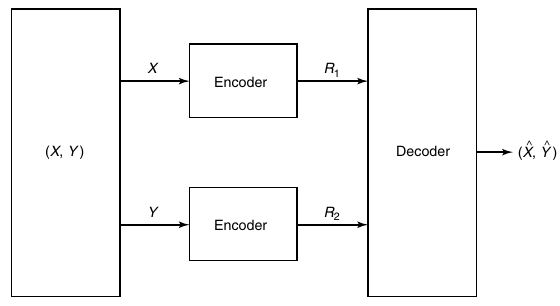
\includegraphics[scale = 0.3]{Diagrams/SWC.png}
\end{center}

 \begin{itemize}
	\justifying

\item<1-> \begin{tcolorbox}[colback=blue!10, colframe=blue, title=Slepian-Wolf Theorem]
For the distributed source coding problem for the source $(X,Y)$ drawn i.i.d. $\sim p(x,y)$, the achievable rate region is given by
%
\begin{eqnarray*}
  R_1 \geq H(X|Y), \text{ } R_2 \geq H(Y|X), \text{ } R_1+R_2 \geq H(X,Y).
\end{eqnarray*}
%
\end{tcolorbox}

  \end{itemize}
\end{frame}

%%%%%%%%%%%%%%%%%%%%%%%%%%%%%%%%%%%%%%%%%%%%%%%%%%%%%%%%%%%%%%%%%%%%
%Frame
\begin{frame}{Examples of Slepian-Wolf Theorem}
 \begin{itemize}
	\justifying

\item<1-> Let us demonstrate the result with an example. Consider $(X,Y)$ have the joint probability mass function $p(x,y)$:
%
\begin{eqnarray*}
   \begin{tabular}{|c|c|c|c|}
        \hline
        \backslashbox{\blue{$X  \downarrow$}}{\red{$Y\rightarrow$ }} & \red{0} & \red{1} \\
       \hline
        \blue{0} & $\frac{1}{3}$ & $\frac{1}{3}$ \\
        \hline
        \blue{1} & 0 & $\frac{1}{3}$ \\
        \hline
    \end{tabular}
\end{eqnarray*}
%

\item<2-> Transmit the sources independently will require $2$ bits. 

\item<3-> Now use Slepain-Wolf encoding.
%
\begin{eqnarray*}
    H(X) = -\sum_{x} p(x)\log p(x) = 0.918 \mbox{ bits},\\
    H(Y|X) = \sum_{x} p(X=x)H(Y|X=x) = 0.667 \mbox{ bits}.
\end{eqnarray*}

\item<4-> Hence, for Slepain-Wolf encoding, we only need 1.584 bits.

	\end{itemize}
\end{frame}

%%%%%%%%%%%%%%%%%%%%%%%%%%%%%%%%%%%%%%%%%%%%%%%%%%%%%%%%%%%%%%%%%%%%
%Frame
\begin{frame}{Rate region for Slepian-Wolf encoding}
 \begin{center}
     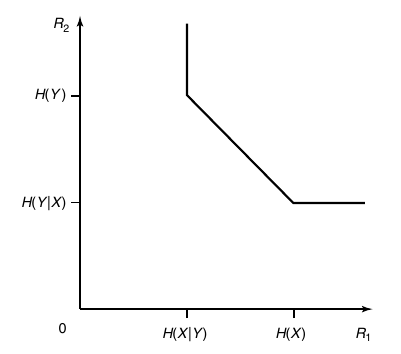
\includegraphics[scale=0.45]{Diagrams/SWE.png}
 \end{center}
\end{frame}

%%%%%%%%%%%%%%%%%%%%%%%%%%%%%%%%%%%%%%%%%%%%%%%%%%%%%%%%%%%%%%%%%%%%
%Frame
\section{BC}
\begin{frame}{Broadcast Channel (A Brief Introduction)}
 \begin{itemize}
	\justifying

\item<1-> A communication channel with one sender and two or more receivers.

\item<2-> The basic problem is finding the set of simultaneously achievable rates for communication in a broadcast channel.

\item<3-> The TV (or radio) station is one of the simplest and most common examples of broadcast channels.
\begin{center}
    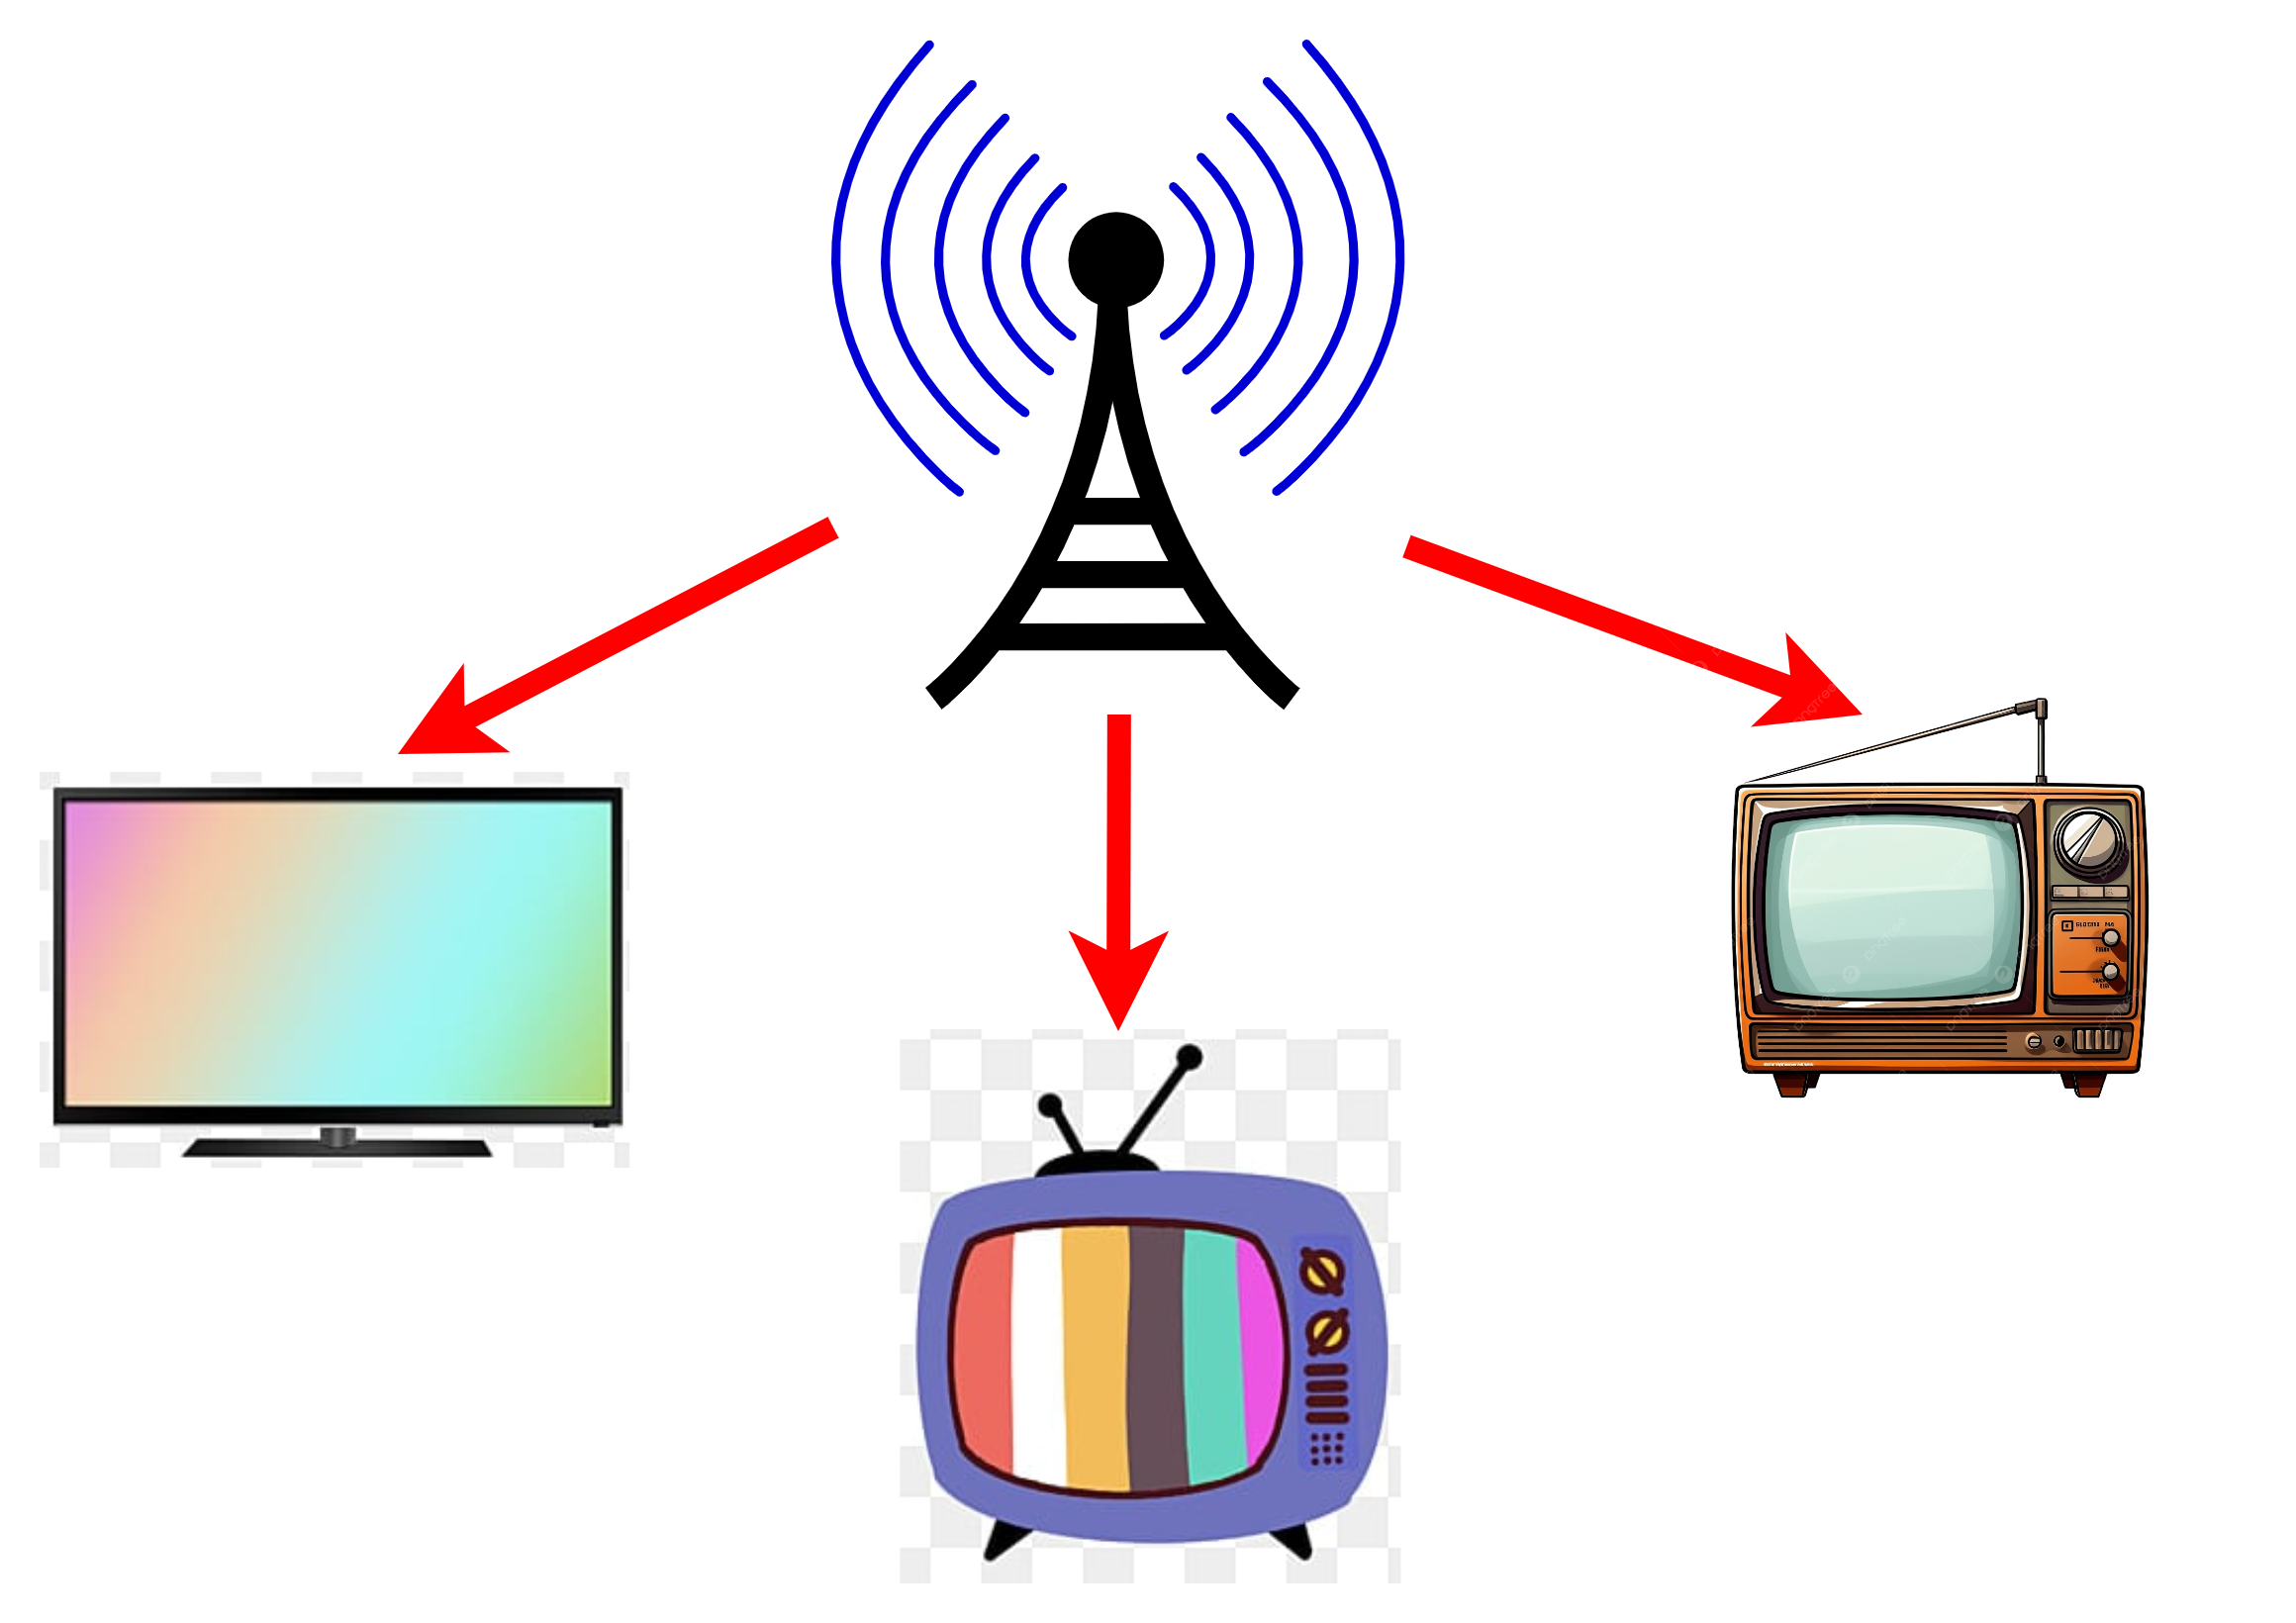
\includegraphics[scale=0.05]{Presentation Diagrams/TVBC.png}
\end{center}
%

	\end{itemize}
\end{frame}






%%%%%%%%%%%%%%%%%%%%%%%%%%%%%%%%%%%%%%%%%%%%%%%%%%%%%%%%%%%%%%%%%%%%
%Frame-4
\section{Future Plans}

\begin{frame}{Future Plans}
 \begin{itemize}
	\justifying

\item<1-> \textbf{\red {Study:}} The Broadcast Channel and The Relay Channel
\item<2-> \textbf{\blue{Research Papers:}}
\begin{itemize}
    \item 1: The Gaussian Erasure Channel \\
    \textit{\tiny Tulino, A., Verdú, S., Caire, G., & Shamai, S. (2007, June). The Gaussian erasure channel. In 2007 IEEE International Symposium on Information Theory (pp. 1721-1725). IEEE.}
    
    
    \item 2: The Two-Tap Input-Erasure Gaussian Channel and its Application to Cellular Communications\\
    \textit{\tiny Somekh, O., Simeone, O., Poor, H. V., \& Shamai, S. (2008, September). The two-tap input-erasure Gaussian channel and its application to cellular communications. In 2008 46th Annual Allerton Conference on Communication, Control, and Computing (pp. 228-235). IEEE.}
\end{itemize}

	\end{itemize}
\end{frame}

%%%%%%%%%%%%%%%%%%%%%%%%%%%%%%%%%%%%%%%%%%%%%%%%%%%%%%%%%%%%%%%%%%
\section*{Bibliography}
%Frame-ending-1
\begin{frame}
\frametitle{Bibliography}
	\begin{thebibliography}{99}
	
\bibitem{cover} Cover, T. M., Thomas, J. A. (2006). Elements of Information Theory 2nd Edition (Wiley Series in Telecommunications and Signal Processing). Wiley-Interscience. ISBN: 0471241954

\bibitem{yeung} Yeung, R. W. (2008). Information theory and network coding. In Springer eBooks. https://doi.org/10.1007/978-0-387-79234-7

\end{thebibliography}

\end{frame}
}
%%%%%%%%%%%%%%%%%%%%%%%%%%%%%%%%%%%%%%%%%%%%%%%%%%%%%%%%%%%%%%%%%%
%Frame-final 
\begin{frame}
\centering
\color{red}\Huge $\mathbb{THANK \quad YOU}$
\end{frame}
%%%%%%%%%%%%%%%%%%%%%%%%%%%%%%%%%%%%%%%%%%%%%%%%%%%%%%%%%%%%%%%%%%


\end{document}